\section{Background of the Study}
%%\Blindtext
	
	A mobile robot is an automatic machine that is fast evolving and has a significant role in the industry. It is capable of moving from one place to another or to execute the program it was given. Some mobile robots have the capability to navigate without the user controlling it, while there are also mobile robots that can be controlled through controllers. Some of its application in the industry includes, manufacturing, agriculture, medical, aerospace and etc. Mobile robots are made up of software, controller, actuators and sensor. Its controller can be made using embedded microcontroller, microprocessor or a computer. Its controller is programmed using assembly language, C, C++ and etc. The kind of sensor that will be equipped in the mobile robot depends on the application. Some application can be for proximity sensing, collision avoidance, positioning, distance calculator and etc. 
	
	The plan is to create a firefighting robot that will be able to extinguish fire and draw the smoke in. It is capable of detecting fire and smoke using a flame sensor and smoke sensor. It can also extinguish the flames by using the small fire extinguisher equipped on it. The mobile robot will be Arduino-based. It will consist of several DC motors.

	The constants will be the battery, the fan, and the room to be used. The goal is to design a system that will allow all components of the robot to function harmoniously. The flame sensor will be integrated with the Arduino to be able to sense the flame and alarm the vehicle. It will approach it and extinguish it using the canister equipped with it.


\section{Prior Studies}
%%Put here a \index{summary}summary of your literature review.  Preferably, a table showing the summary would be helpful. \blindtext

	
	There are many ways to detect fire. As technology improves, ways to detect fire became more and more reliable and accurate. The most reliable fire detectors are still humans because they can see the fire and smell the smoke the moment they appear, which allows them to respond quickly. However, at times when people are not home, electronic fire detectors are needed to keep a house or building safe. One such sensor is the heat detector. According to Science Learning Hub, most heat-detecting sprinklers used these days utilize a fragile glass bulb containing fluid that expands with heat. The glass breaks, spraying water down from the sprinkler. Heat detectors do not cost much and are relatively reliable. They operate completely without electricity as well, which makes them very popular in large establishments. They are, however, slow to respond as the heat needs to reach the ceiling to activate the sprinklers.

	Another way to detect fire is through the use of smoke detectors. Smoke detectors respond faster than heat detectors. They are more sensitive and can respond the moment it detects the smoke from the fire. One drawback of the smoke detector is its complex design and its price. Another drawback is its sensitivity. Sometimes the smoke detector cannot differentiate fire smoke from normal steam or dust.

	Other ways to sense fire include optical flame detectors. These detectors work using ultraviolet or infrared light. Infrared flame detectors sense fire through the infrared spectral band for unique patterns emitted by the hot gas of the flame. However, accuracy of the infrared flame detectors is largely affected when exposed to direct sunlight. Ultraviolet detectors, on the other hand, operate by sensing the UV radiation given off by the flame. These sensors are capable of detecting flames in three to four milliseconds. Between these two optical flame detectors, the UV detector is much more accurate and reliable.

\section{Problem Statement}
%%\blindtext

	
		According to the Philippine Statistics Authority, at least 2,000 fire incidents happen on the months of April to May each year. Fire incidents is one of the major setbacks to the growth of the Philippine’s economy because it does not only do damage to properties, but also result to a sizable number of casualties. With the joint efforts of the Bureau of Fire Prevention (BFP), Red Cross, and other Non-Government Organizations (NGOs), the amount of destruction caused by fires decreased.
    
		However, due to the recent incidents of heavy traffic in Metro Manila, fire and medical volunteers are having a hard time arriving at their destinations. Because of the delayed response of the volunteers, about 2.5 billion pesos worth of property are destroyed, 5,000 civilians left homeless, and 90 persons killed (58 civilians and 32 firefighters) in Metro Manila only. Lack of proper fire response equipment in local barangays also play a part in the destruction caused by the fire.
    
		In response to this problem, The researchers study proposes to create a microcontroller-based mobile robot that can sense and extinguish fire. The said robot can be deployed manually (by a technician) or automatically (by using its flame sensor) to the concerned location. Because the robot will already be placed in the building, the immediate response time to treat the fire will be fairly shorter as compared as to calling the fire department.

\section{Objectives}
\subsection{General Objective(s)}
%%\ldots
\begin{itemized}
	\item To design and to develop a wheeled mobile robot that is capable of detecting fire using an infrared-based flame sensor, and extinguish fire with the use of a small fire extinguisher mounted onto the robot.
\end{itemized}

\subsection{Specific Objectives}

\begin{itemized}
	\item To design and to develop a voltage booster circuit that is capable of powering up a mobile robot carrying a small exhaust fan.;
	
	\item To design and to develop a mobile robot that can detect and locate a flame source.;
	
	\item To develop a mobile robot that is capable of detecting the face of a human within a room with smoke.;

\end{itemized}



\section{Significance of the Study}
%%\blindtext

\textit{People working or living in a building} \newline
	People working or living in buildings that have no complete fire precautions (protection) can use this robot in their daily lives. While the firefighters are still on their way to the rescue, this firefighting robots can clear the smoke from the person’s pathway so he or she won’t suffocate on his or her way out of the vicinity. It can also help people who are trapped in their rooms by extinguishing the flame on small areas using the fire extinguisher equipped on the mobile robot. 

\textit{Fire Fighters} \newline

	This robot can be a great help for firefighters because it can start killing some fires to evacuate the people in a room while the firefighters are on their way to the site or when they are stuck in traffic. It can also lessen the number of deaths among firefighters by letting this robot go into the building to check if there are still small fires or if there are things that are on fire. Furthermore, unmanned vehicles are more suitable for dangerous task to reduce the injuries or even deaths of people.

\textit{School/University} \newline

	This can also give aid in the universities especially in the laboratories where it is possible to have a fire outbreak like chemistry laboratories, electronic laboratories and etc. 

\textit{Selling Point} \newline

	The slightest amount of time during a fire outbreak is very crucial which may decide whether the person will live or die. This mobile robot is designed to help the people in case of a fire in buildings, houses or any closed vicinity, while the firefighters get to the burning site. This mobile robot will not only help the people create a smokeless pathway but will also kill small fires with a mini fire extinguisher equipped. It also lessens injuries and deaths to firefighters since it is an unmanned vehicle.

\section{Assumptions, Scope and Delimitations}

\begin{itemized}
	\item This study will focus on using flame sensors in locating the fire approximately 1 foot away.;
	\item The study will also use an ultrasonic sensors to avoid obstacle and navigate through the room.;
	\item The researchers will use a camera to implement face detection in order to locate victims.;
	\item This study will only cover extinguishing of small scale of fire that have started from non-electrical things.;
	\item The researchers will use an Arduino board as means of communication between the sensors and the motors.;
	\item The researchers will design a battery management module for the robot so the input power will be distributed among the components without making one part of the robot fail or breakdown.;
	\item The mobile robot will not cover fire proofing.;
\end{itemized}

\section{Description and Methodology}

	The project aims to extinguish fire using a wheeled mobile robot equipped with an Arduino, a fire extinguisher, fans, flame sensors, and ultrasonic sensors. The Arduino board acts as the controller of the mobile robot that loads the program that controls the movement of the robot, fans, and sensors which control the fire extinguisher. The board interprets the data sent by the sensors to the microcontroller and loads a specific program which triggers the movement of the robot, the fans, and the fire extinguisher. Since the robot is controlled by sensors, a camera will be mounted in front of the robot to allow the user to see the surroundings and objects in front of it, and detect a human face inside a smokey room.
	
	The research project allows the use of different devices such as fans, camera, sensors, fire extinguisher and a wheeled mobile robot. The researchers would use an algorithm that would allow the mobile robot to navigate through an area and search for fire which it will extinguish while its fans are absorbing the smoke. The research project will then take inputs from the sensor whether the robot should move or not and whether the fan should rotate or not. The camera equipped on the mobile robot will also detect victims of the fire.

	The mobile robot will consist of an Arduino board connected to a motor driver which controls the DC motors. The sensors connected on the mobile robot will consist of the following: ultrasonic sensors, flame sensors, and smoke sensor. The ultrasonic sensor is used by the mobile robot to navigate through the room. The flame sensor is used to locate the flame about a foot apart. The smoke sensor will dictate when the fans will operate in sucking the smoke. The mobile robot will also be equipped with a fire extinguisher which the mobile robot will use in killing the fire. Lastly, the camera will be used in detecting victims of the fire.
	
	The accuracy of the flame sensor can be verified by testing the sensor on set distances from the flame. The flame sensor will first be tested 10 times while placed 3 feet away from the flame; followed by another 10 times, 2 feet away; and finally another 10 times, 1 foot away.
	
\section{Estimated Work Schedule and Budget}
\begin{*table}
\centering
\caption{Estimated Budget}
\label{my-label}
\begin{tabular}{lllll}
Item                            & Quantity & Price (PHP) &  &  \\
Arduino UNO (GizDuino Board)    & 1        & 400         &  &  \\
Bluetooth Camera                & 1        & 430         &  &  \\
Flame Sensor                    & 3        & 135         &  &  \\
Ultrasonic Sensor               & 3        & 750         &  &  \\
Smoke Sensor                    & 1        & 500         &  &  \\
Used Exhaust Fan                & 2        & 400         &  &  \\
Battery                         & 2        & 300         &  &  \\
Buzzer                          & 1        & 15          &  &  \\
Used RC Car                     & 1        & 500         &  &  \\
Fire Extinguisher               & 1        & 195         &  &  \\
DC to DC Booster                & 1        & 140         &  &  \\
Battery Management System Board & 1        & 500         &  &  \\
Total                           & 4265     &             &  & 
\end{tabular}
\end{table}
Figure 1. Estimated Budget

\begin{*figure}
	\centering
	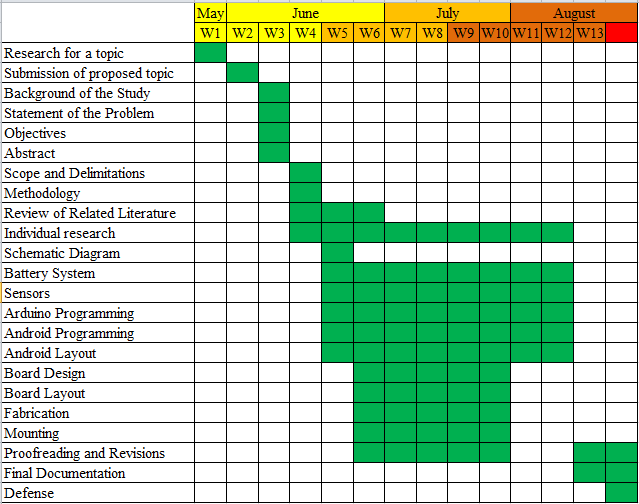
\includegraphics[width=\columnwidth]{GANTT}
	\caption{Figure 2. Gantt Chart}
	\label{fig:fig2}
\end{figure}
Figure 2. Gantt Chart

\begin{*figure}
	\centering
	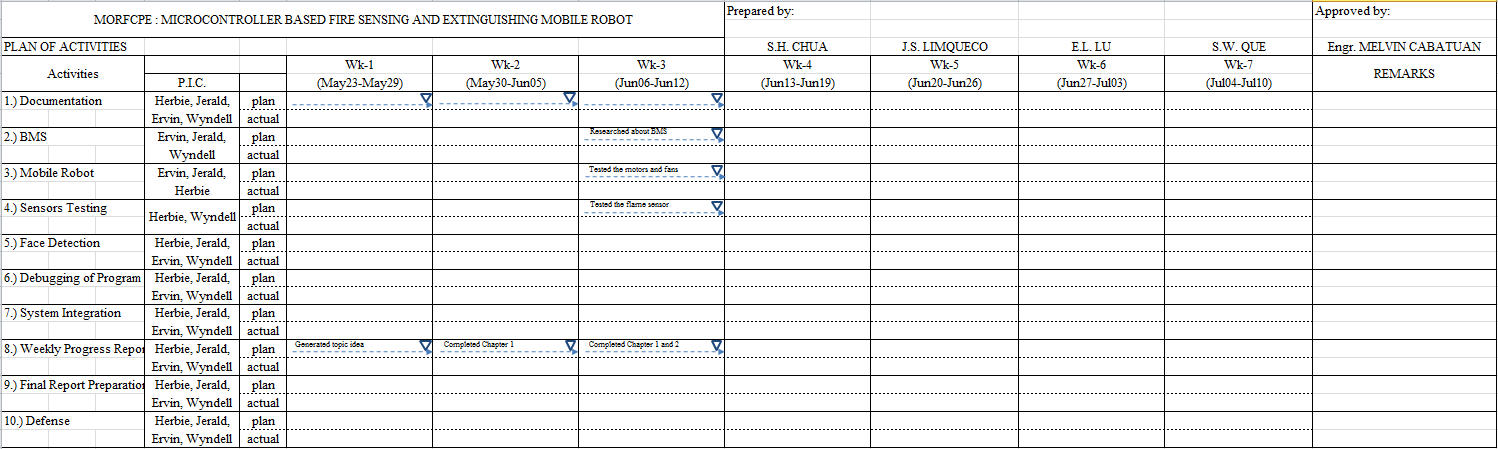
\includegraphics[width=\columnwidth]{WORKPLAN}
	\caption{Figure 3. Workplan}
	\label{fig:fig3}
\end{figure}
Figure 3. Workplan

%%\blindtext

%%\section{Publication Plan}
%%\blindtext

%%\fi


\section{Overview}

	This paper shows how the researchers designed a firefighting mobile robot. It contains all the necessary informations needed to build the robot. The first chapter includes a description of the specifications and functions of the mobile robot. It also has prior studies about the topic that the researchers used to design the robot. The following chapters will cover the research undergone by the researchers to explore the possibilities attainable by the robot through academic articles.

